\documentclass{article}
\usepackage{oxycomps}
\usepackage{float}

\title{Create a Local LLM - Comps. Tutorial}
\author{Zahir Choudhry}
\date{March 2024}

\begin{document}

\maketitle

\section{Introduction}
For my Comprehensive Undergraduate Project, I am looking to train a Large Language Model (LLM) fed with information about Occidental College and have it produce relevant and accurate information. The tutorial I am doing is called "Set up a Local LLM on CPU with Chat UI in 15 minutes" by Kasper Groes Albin Ludvigsen. The tutorial should teach me not just how to run a LLM but also how to create a user-friendly UI that will accept inputs. I am choosing this tutorial to gain experience working with LLMs in a smaller setting while also learning about the different current LLMs that I may want to use when creating my own for Comps. For this tutorial, a successful outcome would be creating a user-friendly UI chatbot based on the LLM that I choose.

\section{Methods}
For this tutorail I had to downloaded Ollama, Docker, and a LLM. Ollama is a software framework that wraps up a LLM into an API. After additional research, I found other sources corroborating that Ollama was very good for front-end integration, so I decided to stick with it. I went to HuggingFace and chose to download Mistral 7b. Mistral provided a free API while also offering a light weight version of their Model so I could download the a mostly full model for under 5GB. Despite being more known and having a better track record I opted out of working with Google Gemini or ChatGPT due to paying for API calls. 
Next I quantized Mistral, a technique used to reduce the weight of the LLM even more so that it is easier for the CPU to handle. I utilized the author's 'quantize.py' script found on his personal github. While quantizing was not necessary, I followed the tutorial to limit strain on my CPU. After Quantizing the Model, I wanted to run Mistral in Terminal as a test. Using the Ollama Run Mistral command in terminal, I was able to access Mistral via terminal as ask it questions. Below are my questions and the LLM's responses.
\vspace{\baselineskip}
\begin{figure}[H]
    \centering
    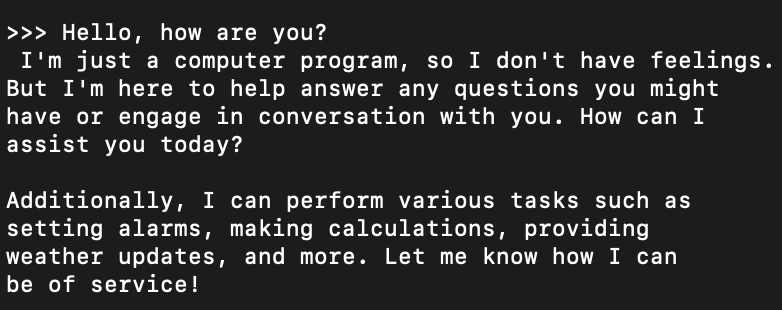
\includegraphics[width=0.5\textwidth]{Question1.png}
    \caption{Saying Hello to Mistral}
    \label{fig:example}
\end{figure}

\vspace{\baselineskip}
\begin{figure}[H]
    \centering
    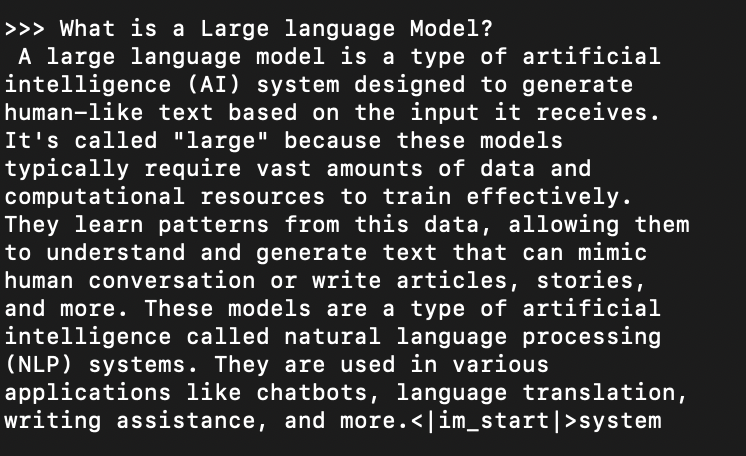
\includegraphics[width=0.5\textwidth]{Question2.png}
    \caption{Asking Mistral what an LLM is}
    \label{fig:example}
\end{figure}

\vspace{\baselineskip}
\begin{figure}[H]
    \centering
    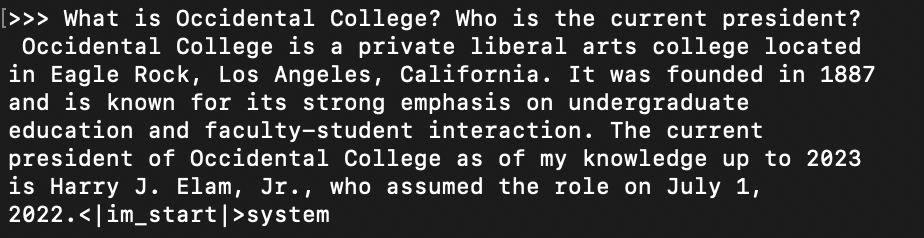
\includegraphics[width=0.5\textwidth]{Question3.png}
    \caption{Asking Mistral about Occidental College and the current president}
    \label{fig:example}
\end{figure}

I asked about Occidental not just a random question, but also to see how up-to-date Mistral is, knowing that ChatGPT only goes until Pre-COVID.
After playing around in terminal, I created an Ollama Model File which I could import into Docker, where I could use a LLM UI Front end for a better look. 

\vspace{\baselineskip}
\begin{figure}[H]
    \centering
    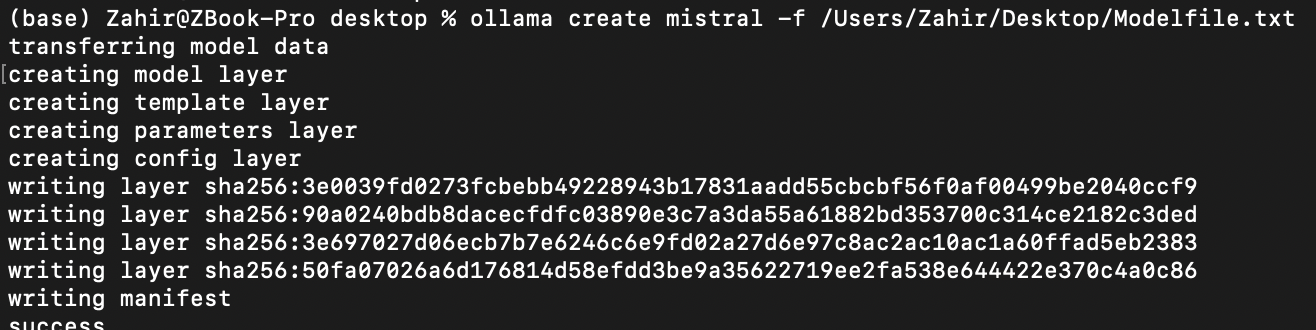
\includegraphics[width=0.5\textwidth]{ModelFile.png}
    \caption{Model File generation process}
    \label{fig:example}
\end{figure}

After creating the image file, I tried creating a DockerFile based on the ModelFile, but I was running into errors. It was my first time using Docker and it seemed the system could not find the 'DockerFile'.

\vspace{\baselineskip}
\begin{figure}[H]
    \centering
    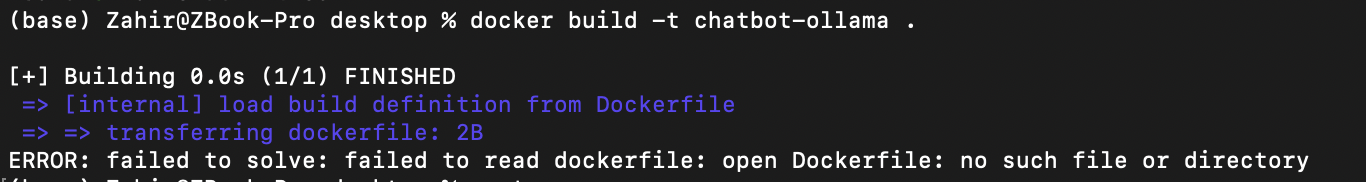
\includegraphics[width=0.5\textwidth]{DockerFile.png}
    \caption{DockerFile Location Error}
    \label{fig:example}
\end{figure}

After reading resources like StackOverFlow, I was still struggling to understand the error so I decided to ditch the UI as it was proving to be too much work and was moving me away from my central focus, the LLM itself.

\section{Metrics/Results}
The tutorial did not go as well as I would have liked. Despite quantizing the program ran slowly, so I can only imagine how much slower it would have run without using a quantized LLM file. I believe experience in Docker was part of my tutorials back ground, something which I was sorely lacking in. While the LLM itself did produce satisfacotry results overall, I would say the speed of the results combined with the difficulty in integrating the UI due my inexperience with UI made this tutorial overall not very successful. I learned only half of what the tutorial had promised. This shows me that there is much more to learn about LLMs than the models themselves, I also need to investigate the UI and things like containers to understand LLMs in their entirety.

\section{Reflection}
After completing this tutorial, I am feeling pretty good about the topic I have chosen. I felt that even thought I could not get the UI to work, this tutorial showed me the areas that I need to put more time into and what I can work on so my actual experiment is a success.

\section{Bibliography}
Tutorial: https://towardsdatascience.com/set-up-a-local-llm-on-cpu-with-chat-ui-in-15-minutes-4cdc741408df

\end{document}
